\phantomsection

\chapter{\uppercase{EVALUATION OF THE DECEPTION DETECTION CAPABILITIES OF LLMS IN
MULTIMODAL SETTINGS}}


\section{List of Non-verbal Features}
\label{non-verbal}
RLTD dataset comes with a set of 40 manually annotated non-verbal features. These features are broadly categorized into \textit{facial displays} and \textit{hand movements}. The original annotation provides a binary value for each of these features with respect to whether these attributes were demonstrated by the primary speaker in the video. We filter the most relevant 16 features and use the feature names directly for generating LLM predictions. A list of these features is - \texit{Both Hands Movement, Complex Hands Trajactory, Downwards Lip Movement, Eyes Closing Repeatedly, Frown, Gaze Down, Gaze Side, Gaze at Interlocutor, Head Down, Mouth Closed, Mouth Opened, Raise Eyebrows, Repeated Nods, Scowl, Single Hand Movement, Upwards Lip Movement}.

\section{Response Generation Strategies}
\label{reasoning gen}


\begin{table}[ht]
\centering
\small
% \resizebox{\columnwidth}{!}{
\begin{tabular}{l c c cc cc cc}
\toprule
\textbf{LLM} & \textbf{Config} & \textbf{Response}
  & \multicolumn{2}{c}{\textbf{RLTD}}
  & \multicolumn{2}{c}{\textbf{MU3D}}
  & \multicolumn{2}{c}{\textbf{OpSpam}} \\
\cmidrule(lr){4-5}\cmidrule(lr){6-7}\cmidrule(lr){8-9}
 & & \textbf{Generation} & \textbf{Acc} & \textbf{F1}
     & \textbf{Acc} & \textbf{F1}
     & \textbf{Acc} & \textbf{F1} \\
\midrule

% -----------------------
% Llama-3.1-8B
% -----------------------
\multirow{4}{*}{LLaMA 3.1} 
 & \multirow{2}{*}{zero shot} 
   & label 
     &  54.67 & 51.00
     &  49.61 & 48.51
     &  52.35 & 52.33 \\
 & 
   & label + reasoning 
     & 52.07 & 50.27 
     & 48.44 & 47.95 
     & 51.18 & 51.17 \\
\cmidrule(lr){2-9}
 & \multirow{2}{*}{few shot}
   & label
     & 68.87 & 68.14 
     & 51.72 & 51.18 
     & 59.62 & 59.19 \\
 &
   & label + reasoning
     & 65.71 & 65.61
     & \textbf{56.49} & \textbf{56.15} 
     & 61.43 & 60.83 \\
\midrule

% -----------------------
% Gemma2-9B
% -----------------------
\multirow{4}{*}{Gemma 2} 
 & \multirow{2}{*}{zero shot} 
   & label 
     & 67.77 & 66.67
     & 52.35 & 48.20 
     & 49.28 & 48.45 \\
 & 
   & label + reasoning
     & 66.12 & 64.20
     & \underline{55.63} & \underline{54.42}
     & 50.28 & 47.00 \\
\cmidrule(lr){2-9}
 & \multirow{2}{*}{few shot}
   & label
     & \underline{69.63} & \underline{69.52} 
     & 54.22 & 52.34 
     & 57.70 & 57.59 \\
 &
   & label + reasoning
     & 68.18 & 68.00 
     & 53.91 & 50.73
     & 59.68 & 57.75 \\
\midrule

% -----------------------
% GPT-4o
% -----------------------
\multirow{4}{*}{GPT-4o} 
 & \multirow{2}{*}{zero shot}
   & label 
     & 67.63 & 67.62 
     & 52.42 & 43.98
     & 58.53 & 53.72 \\
 & 
   & label + reasoning
     & 64.46 & 64.31
     & 51.41 & 41.89 
     & 59.04 & 53.63\\
\cmidrule(lr){2-9}
 & \multirow{2}{*}{few shot}
   & label
     & \textbf{71.69} & \textbf{71.39} 
     & 53.20 & 46.86 
     & \textbf{68.40} & \textbf{67.58} \\
 &
   & label + reasoning
     & \underline{69.63} & 69.07 
     & 52.17 & 42.67
     & \underline{64.20} &  \underline{61.04}\\
\bottomrule
\end{tabular}
% }
% \captionsetup{font=footnotesize}
\caption{Comparison of different response generation strategies (direct label prediction vs.\ post-hoc reasoning generation) under zero-shot and few-shot settings. The few-shot examples are randomly selected. The best and second best results are indicated by \textbf{bold} and \underline{underline} respectively.}
\label{tab:response_generation_shots}
\end{table}

The results in Table~\ref{tab:response_generation_shots} offer a comparative analysis between direct label prediction and post-hoc reasoning generation across the three datasets. We systematically evaluate whether generating reasoning after the label contributes positively to the model’s predictive performance, under both zero-shot and few-shot prompting settings. Across most of the settings, particularly on RLTD dataset, direct label prediction tends to yield higher accuracy and F1 scores. For example, GPT-4o achieves an F1 score of 71.39 on RLTD with few-shot direct label prediction, outperforming its label+reasoning counterpart (69.63 F1 score). However, this trend does not hold universally. In the MU3D dataset, which involves scripted deception, post-hoc reasoning occasionally matches or slightly improves performance. LLaMA 3.1, for instance, reaches its best F1 score of 56.15 on MU3D using few-shot post-hoc reasoning. In the OpSpam dataset, dominated by textual content, the advantage again leans toward direct label prediction. GPT-4o in particular shows a noticeable drop in F1 score from 67.58 (few-shot label) to 61.04 (few-shot label + reasoning), suggesting that the inclusion of generated explanations may introduce noise or ambiguity, especially when no visual or behavioral cues are available to ground the reasoning. While post-hoc reasoning generation provides interpretability of model predictions, it does not consistently improve classification performance, and in many cases, leads to modest degradation. 

\section{Performance Trends in Few-Shot Learning}
\label{sec:llm_nshots}
In our study, we examined how large language models (LLMs) perform across various datasets using few-shot prompting. We calculated the F1 score by averaging results across all seeds to ensure consistent measurement as illustrated in Figure ~\ref{fig:llm_shots}. Our findings reveal that models like GPT-4o initially improve with more few-shot examples, demonstrating their ability to use additional data effectively. However, this improvement subsequently declined when too many examples were provided, likely due to the increased complexity of the prompts complicating the model's reasoning ability. LLaMA 3.1 consistently showed significant gains with an increased number of examples for OpSpam and MU3D, indicating strong adaptability to more extensive data inputs. Gemma 2's performance improved on the OpSpam dataset with more examples but declined on the MU3D and RLTD datasets after a certain point. This pattern suggests a possible optimization ceiling, where additional examples no longer contribute to performance enhancements and may instead hinder the model's effectiveness due to prompt saturation.

\begin{figure*}
    \centering
    \includegraphics[width=0.90\textwidth]{images/dc_num_shots.png}
    \captionsetup{font=scriptsize}
    \caption{F1 score across n-shots in few shot learning}
    \label{fig:llm_shots}
\end{figure*}


\section{LLM Reasoning Analysis Examples}
We have illustrated several examples on the basis of deception cues across three datasets in  Figure \ref{fig:llm_reason1}, Figure \ref{fig:llm_reason2}.
\label{sec:llm_ra}

\begin{figure*}
    \centering
    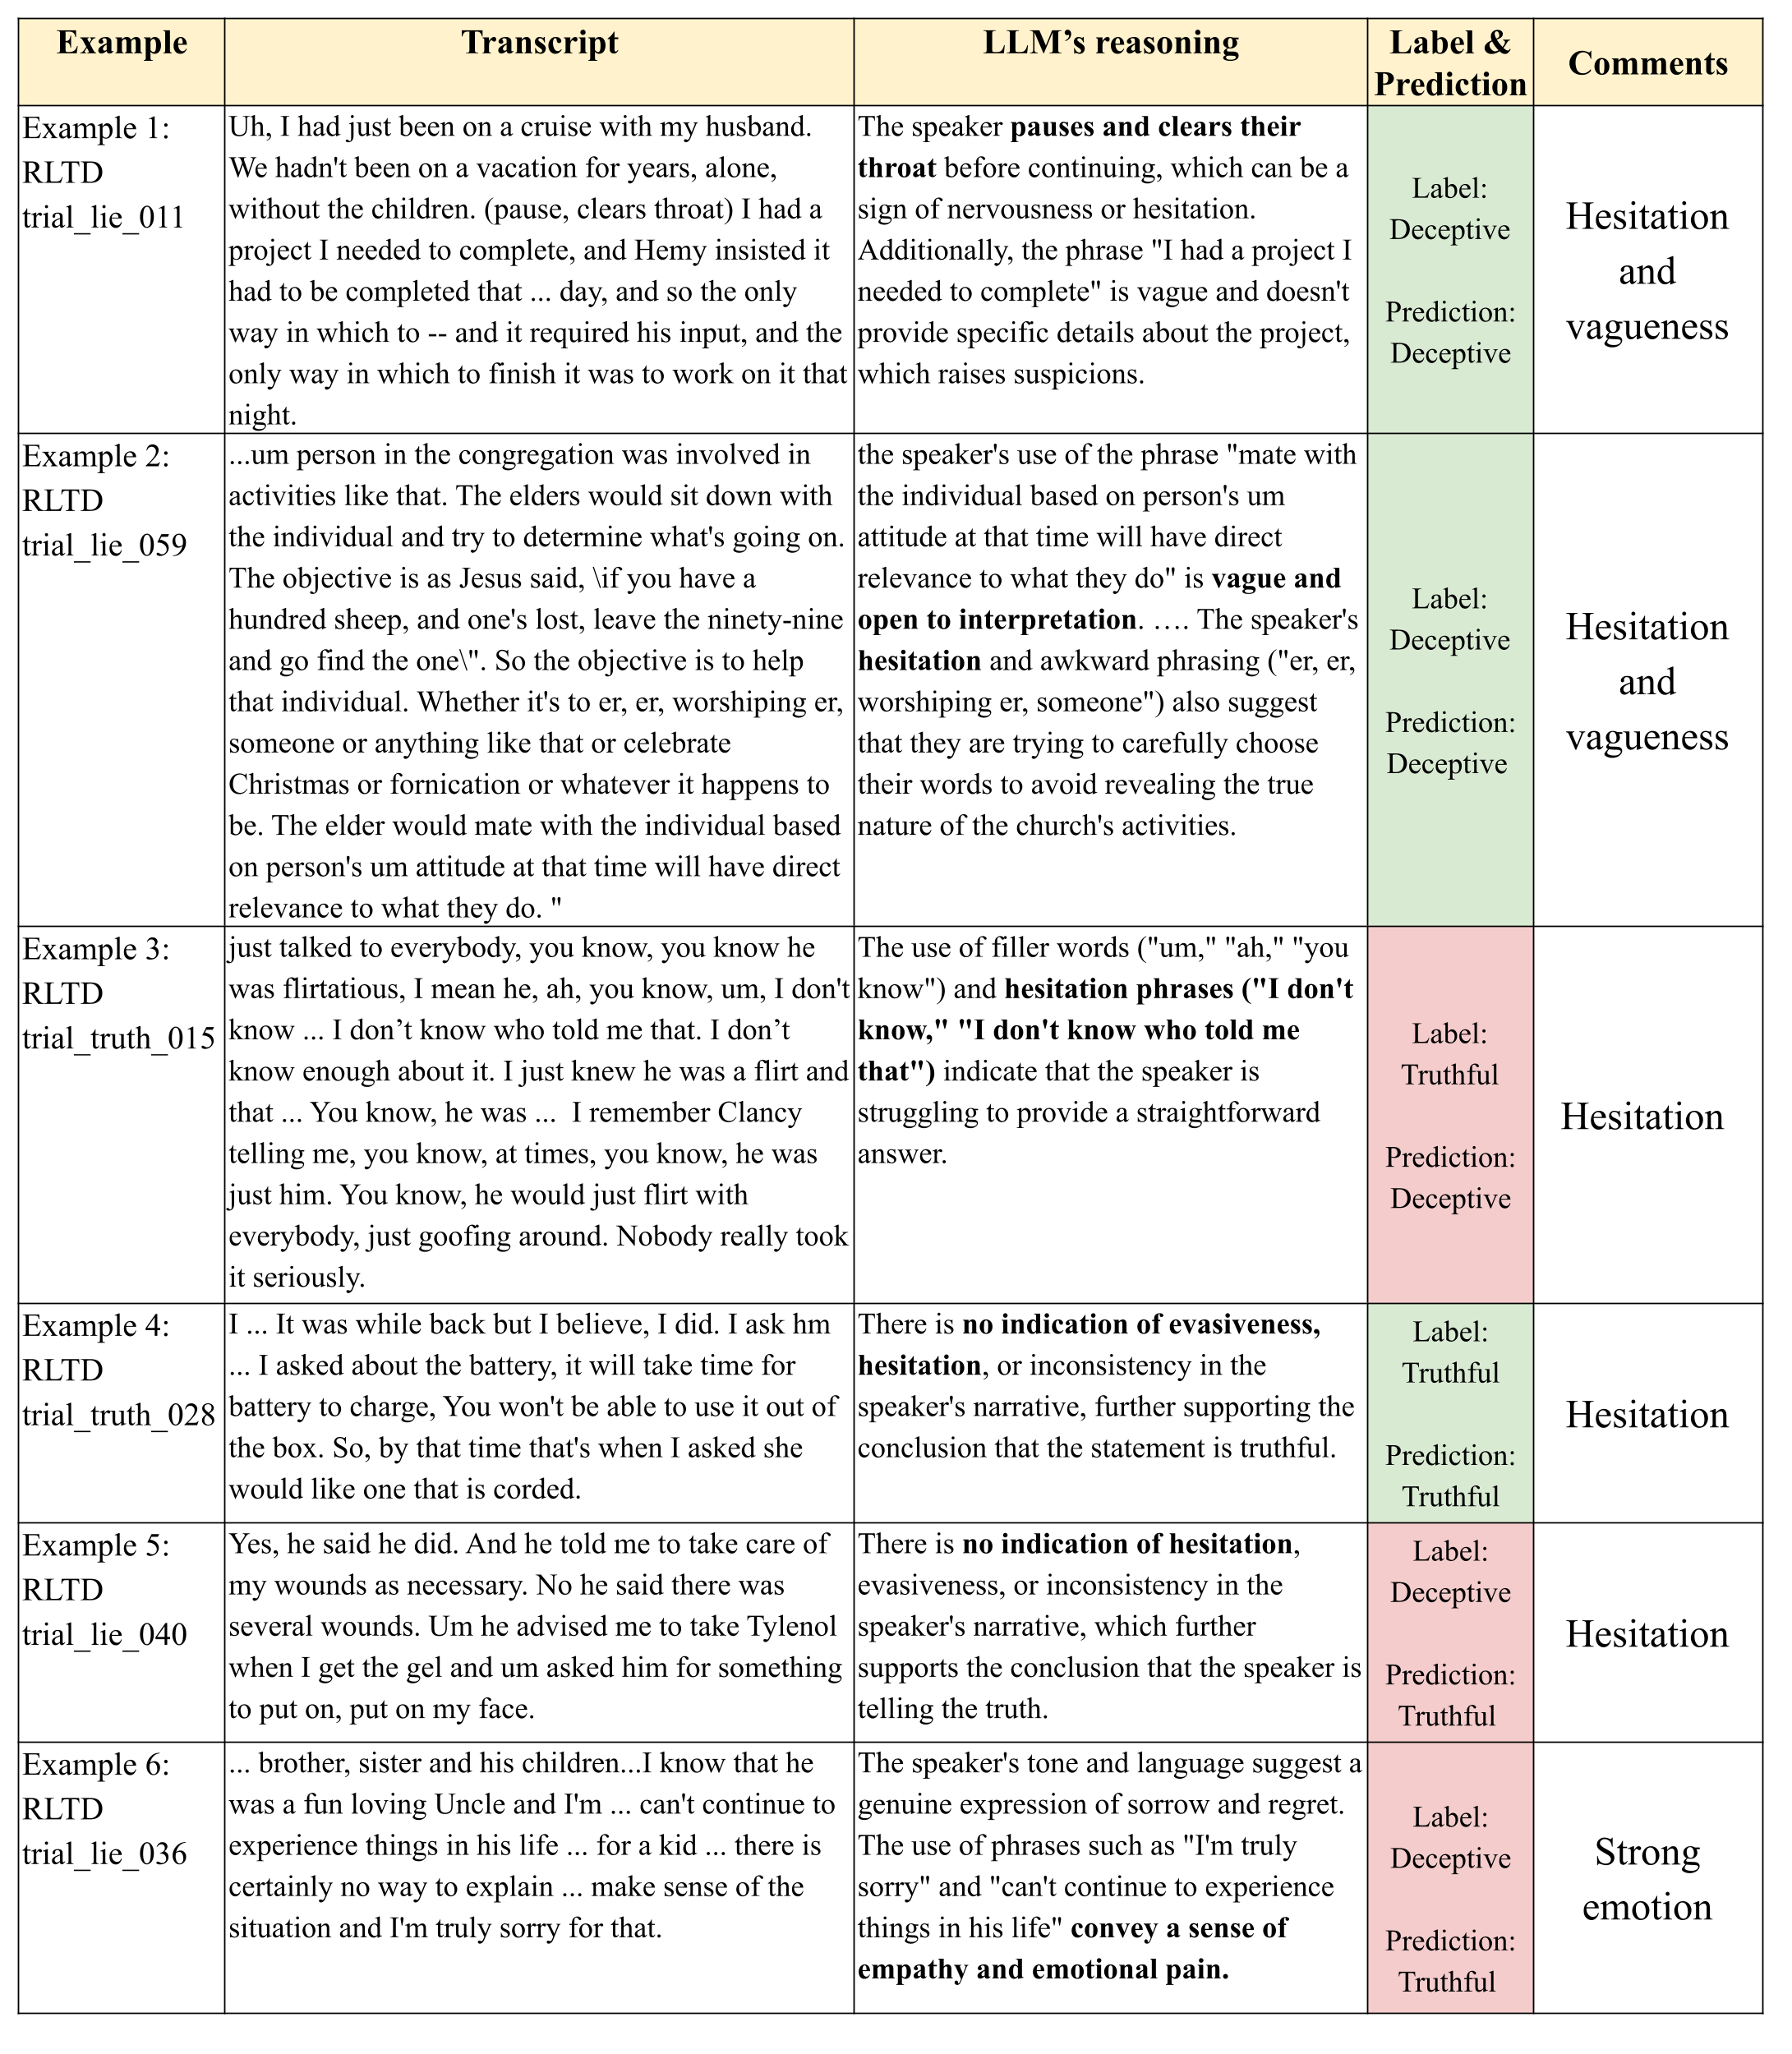
\includegraphics[width=1\textwidth]{images/dc_Deception_1.png}
    \captionsetup{font=scriptsize}
    \caption{Examples of LLM Reasoning on RLTD Dataset}
    \label{fig:llm_reason1}
\end{figure*}


\begin{figure*}
    \centering
    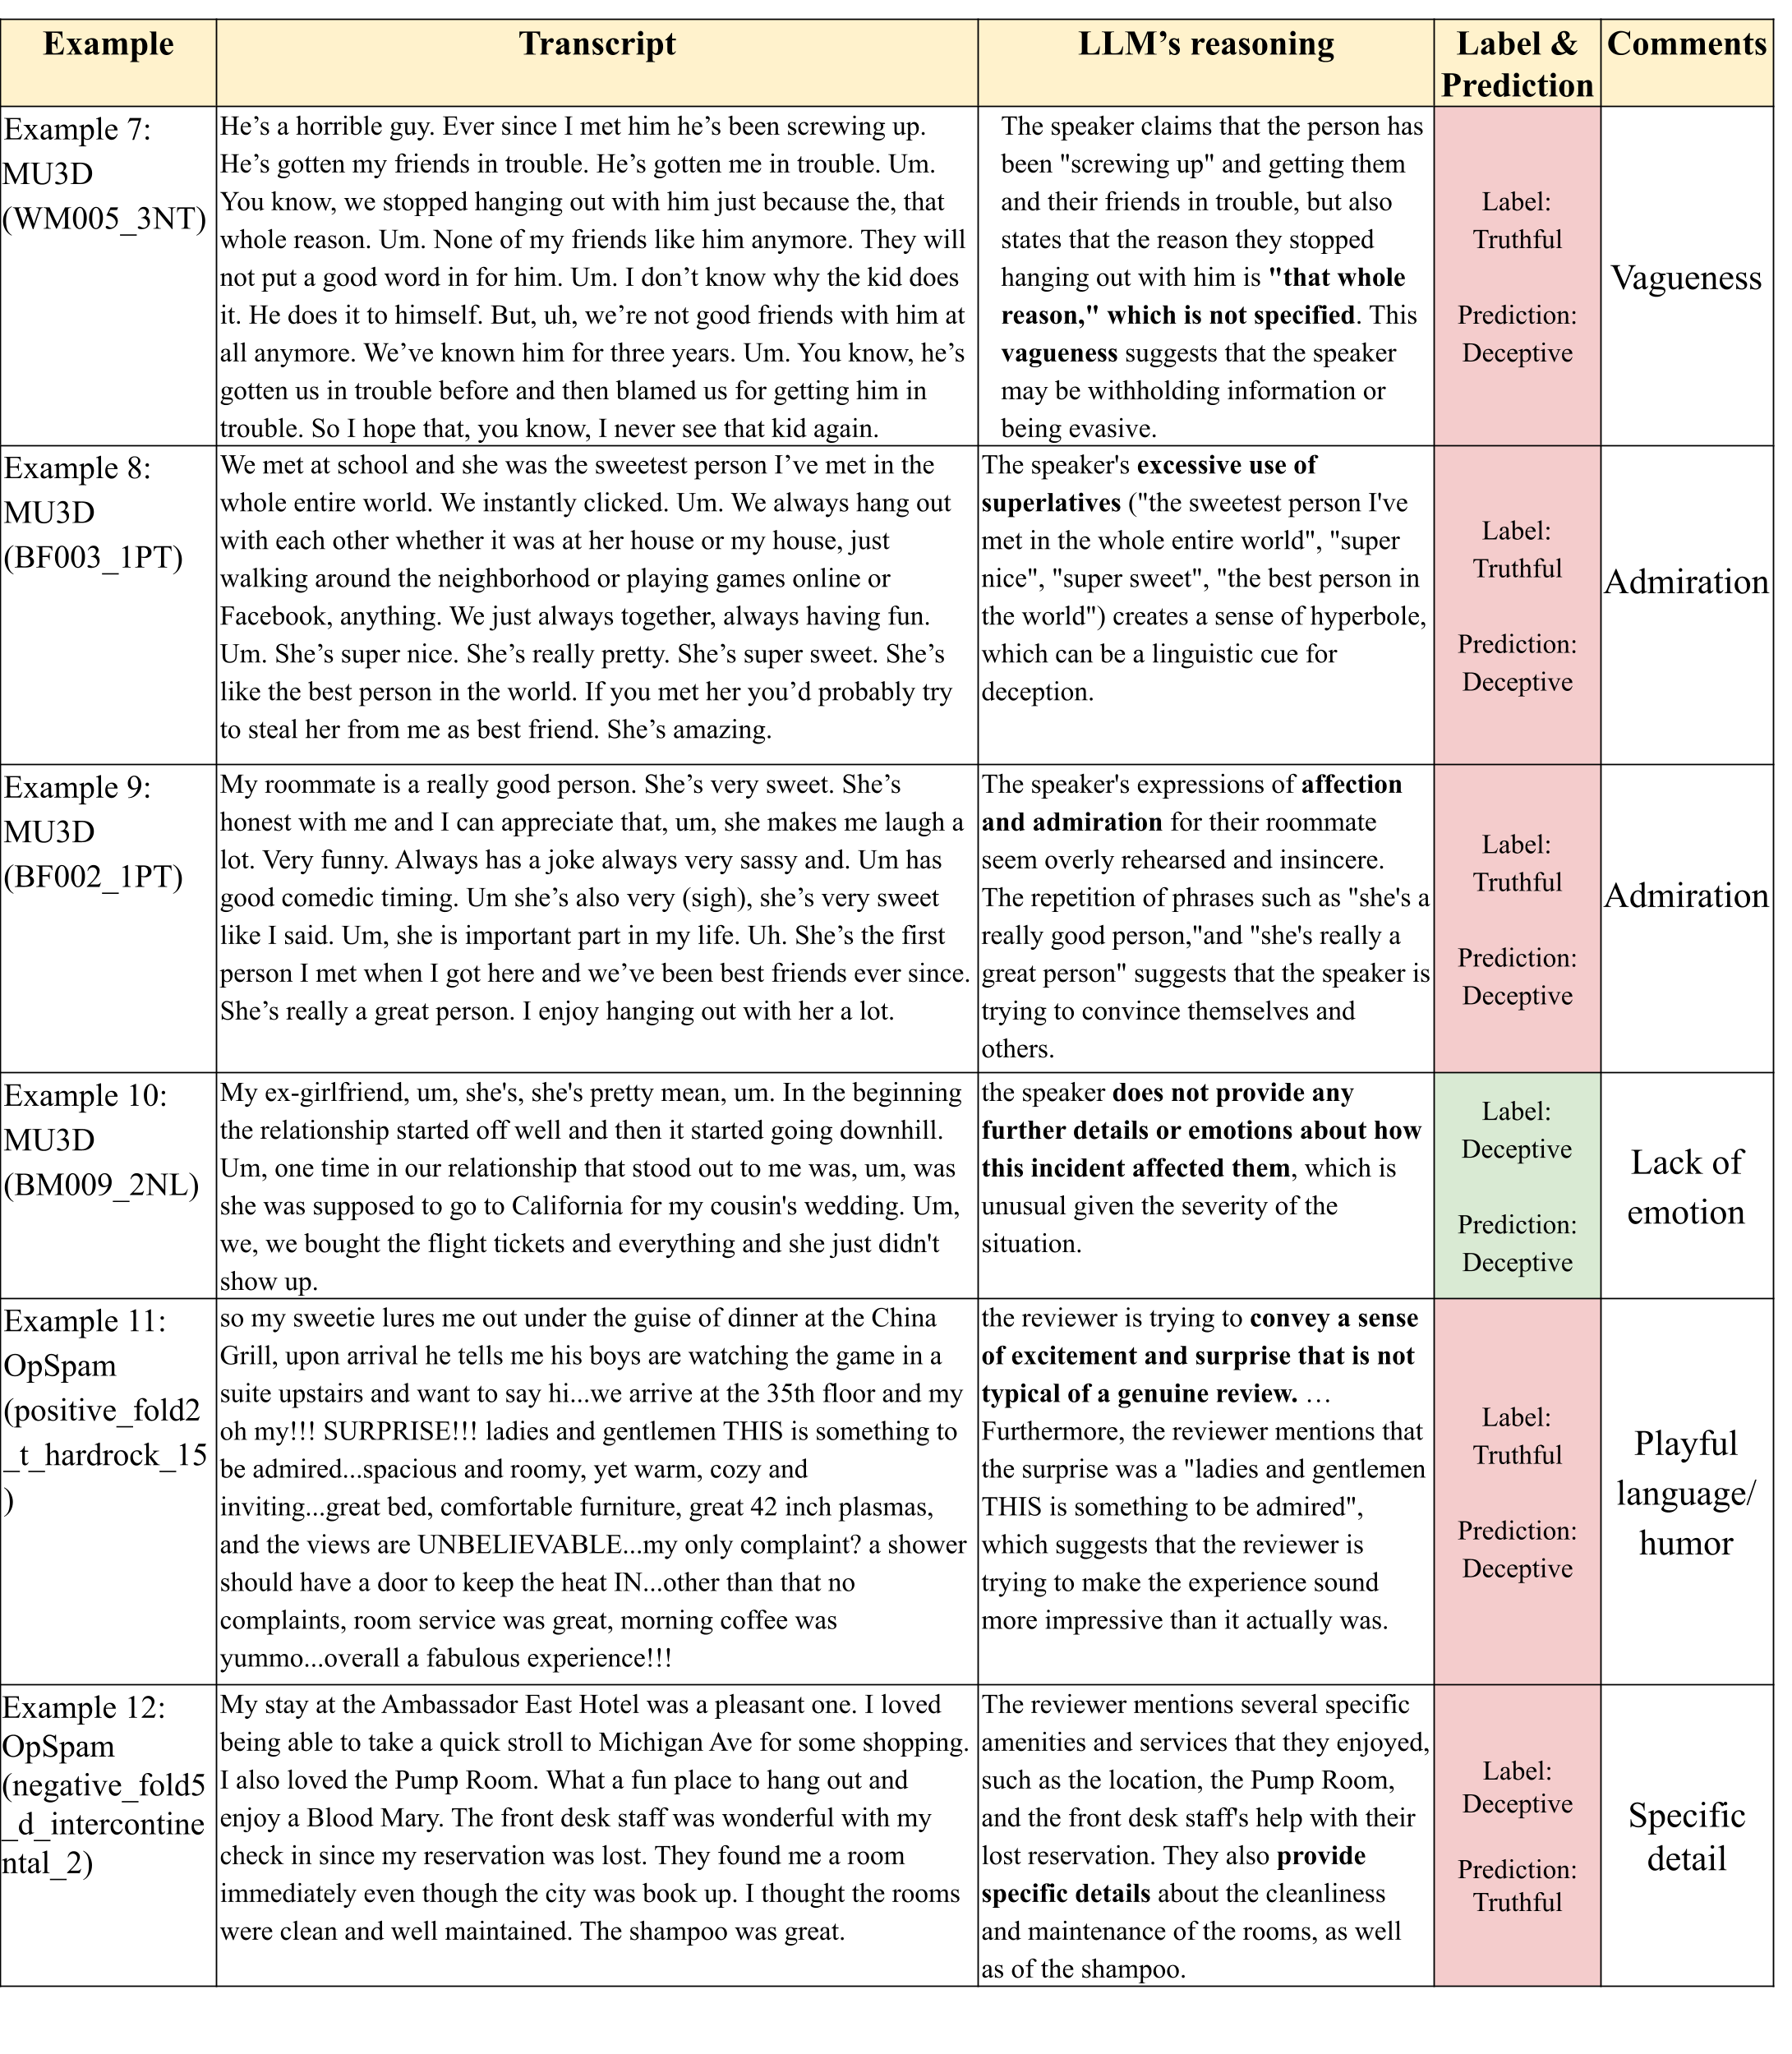
\includegraphics[width=1\textwidth]{images/dc_Deception_2.png}
    \captionsetup{font=scriptsize}
    \caption{Examples of LLM Reasoning on MU3D and OpSpam Dataset}
    \label{fig:llm_reason2}
\end{figure*}

\section{Post-hoc Reasoning Generation vs Chain-of-Thought Reasoning}
\label{cot}

\begin{table}
\centering
\small
\begin{tabular}{l c cc cc cc}
\toprule
% -- First header row --
\textbf{LLM} 
  & \textbf{Order}
  & \multicolumn{2}{c}{\textbf{RLTD}}
  & \multicolumn{2}{c}{\textbf{MU3D}}
  & \multicolumn{2}{c}{\textbf{OpSpam}} \\
\cmidrule(lr){3-4}\cmidrule(lr){5-6}\cmidrule(lr){7-8}
% -- Second header row --
 & 
 & \textbf{Acc} & \textbf{F1}
 & \textbf{Acc} & \textbf{F1}
 & \textbf{Acc} & \textbf{F1} \\
\midrule

% ---- LLaMA 3.1 ----
\multirow{2}{*}{LLaMA 3.1} 
  & \textit{l $\rightarrow$ r}    & 65.71 & 65.61 & 56.49 & 56.15 & 61.43 & 60.83 \\
  &\textit{r $\rightarrow$ l}    & 58.13 & 55.31 & 52.08 & 49.50 & 58.60 & 57.62 \\
\midrule

% ---- Gemma 2 ----
\multirow{2}{*}{Gemma 2} 
  & \textit{l $\rightarrow$ r}    & 68.18 & 68.00 & 53.91 & 50.73 & 59.68 & 57.75 \\
  & \textit{r $\rightarrow$ l}    & 58.68 & 54.39 & 50.63 & 50.39 & 61.62 & 59.36 \\
\bottomrule
\end{tabular}
% \captionsetup{font=scriptsize}
\caption{Comparison of LLM performances under different reasoning generation orderings across datasets. \textit{l $\rightarrow$ r}: label $\rightarrow$ reasoning; \textit{r $\rightarrow$ l}: reasoning $\rightarrow$ label.}
\label{tab:cot}
\end{table}


While generating additional reasoning for predicted labels, we adopt a \textbf{post-hoc reasoning generation} strategy, where the model first outputs the classification label, followed by a justification. An alternative is \textbf{chain-of-thought reasoning}, where the model first reasons over the input before predicting the final label. We chose the post-hoc approach based on empirical evidence. Specifically, we conducted a controlled comparison of the two prompting strategies — (a) label $\rightarrow$ reasoning (post-hoc) and (b) reasoning $\rightarrow$ label (chain-of-thought)—under a few-shot setting across three datasets. As shown in Table~\ref{tab:cot}, the post-hoc reasoning generation strategy generally outperforms chain-of-thought.

In addition to the performance improvements, the post-hoc reasoning reasoning strategy offers better interpretability for analyzing LLM's decision making process. When reasoning is generated prior to the label, LLMs often produce explanations that weigh cues supporting both possible classes. This makes it difficult to use the generated reasoning to interpret the model’s decision, as it lacks a clear alignment with the predicted label. An example of LLM prediction through chain-of-thought -

\textit{ \textbf{Reasoning:} 1. The speaker starts with "Ah, I don't remember," which is a common phrase used when someone is unsure or trying to downplay their memory of an event. This could be a sign of deception, but it's not conclusive on its own.
2. The speaker then says "evidently I, I -- I tried to call Hemy," which is a vague statement. The use of "evidently" suggests that the speaker is not entirely sure about their actions, and the repetition of "I" creates a sense of hesitation.
[...] 6. Overall, the speaker's statements seem inconsistent and vague, which could be a sign of deception. However, the timeline could suggest truthfulness.
\textbf{Judgment:} Deceptive}

In this case, the reasoning incorporates both pro-truthful and pro-deceptive cues before arriving at a final judgment. Hence, it becomes challenging to systematically identify which cues LLMs rely on most frequently for decision-making at scale. In contrast, the post-hoc reasoning generation strategy leads to more focused, label-aligned justifications that are easier to interpret and trace back to specific cues - 

\textit{\textbf{Reasoning:} The speaker claims they tried to call Hemy (presumably their boss) to inform them that they had left the office and something had happened to their husband. However, the speaker immediately follows this statement with "Which seemed -- was a very normal thing for me to have done." This phrase suggests an attempt to justify or rationalize their actions, which is a common linguistic cue for deception. Additionally, the speaker's initial claim "I don't remember" followed by a detailed account raises a red flag, indicating they may be filling in memory gaps with plausible details.
\textbf{Judgment:} Deceptive
}

Based on both empirical evidence and interpretability advantages, we adopt the post-hoc reasoning generation approach over chain-of-thought prompting.
